\documentclass[11pt,a4paper]{article}
\usepackage[margin=2.5cm]{geometry}
\usepackage{graphicx}
\usepackage{xcolor}
\usepackage{tikz}
\usepackage{amssymb}
\usepackage{enumitem}
\usepackage{tcolorbox}
\usepackage{fancyhdr}

% Only 3 colors - much simpler palette
\definecolor{primaryblue}{HTML}{1f77b4}
\definecolor{secondarygray}{HTML}{7f7f7f}
\definecolor{accentorange}{HTML}{ff7f0e}

% Page style
\pagestyle{fancy}
\fancyhf{}
\lhead{\textcolor{primaryblue}{\textbf{Discovery Journey}}}
\rhead{\textcolor{secondarygray}{Before We Begin}}
\cfoot{\thepage}
\renewcommand{\headrulewidth}{0.4pt}
\setlength{\headheight}{14pt}

% Simple box environment
\newtcolorbox{discoverybox}{
    colback=white, 
    colframe=primaryblue, 
    boxsep=8pt,
    arc=0pt,
    boxrule=1.5pt
}

\newtcolorbox{observebox}{
    colback=white, 
    colframe=secondarygray, 
    boxsep=8pt,
    arc=0pt,
    boxrule=1pt
}

\begin{document}

% PAGE 1: Simple Cover without name fields
\thispagestyle{empty}
\begin{center}
\vspace*{2cm}

{\Huge \textcolor{primaryblue}{\textbf{Discovering Patterns}}}

\vspace{1cm}

{\LARGE \textcolor{secondarygray}{What you'll discover before we begin}}

\vspace{2cm}

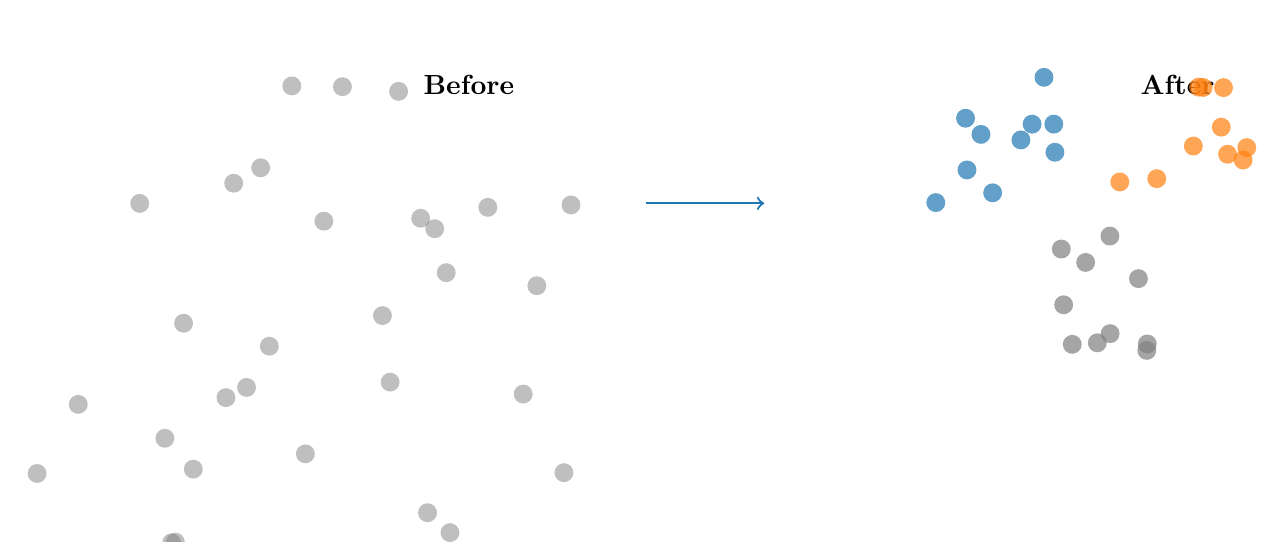
\begin{tikzpicture}[scale=1.5]
% Before: Random dots
\node at (-3, 2) {\textbf{Before}};
\foreach \i in {1,...,30}
{
    \pgfmathsetmacro{\xpos}{rand*2.5-4.5}
    \pgfmathsetmacro{\ypos}{rand*2}
    \fill[secondarygray,opacity=0.5] (\xpos,\ypos) circle (0.08);
}

% Arrow
\draw[->,thick,primaryblue] (-1.5,1) -- (-0.5,1);

% After: Organized groups
\node at (3, 2) {\textbf{After}};
% Group 1
\foreach \i in {1,...,10}
{
    \pgfmathsetmacro{\xpos}{rand*0.6+1.5}
    \pgfmathsetmacro{\ypos}{rand*0.6+1.5}
    \fill[primaryblue,opacity=0.7] (\xpos,\ypos) circle (0.08);
}
% Group 2
\foreach \i in {1,...,10}
{
    \pgfmathsetmacro{\xpos}{rand*0.6+3}
    \pgfmathsetmacro{\ypos}{rand*0.6+1.5}
    \fill[accentorange,opacity=0.7] (\xpos,\ypos) circle (0.08);
}
% Group 3
\foreach \i in {1,...,10}
{
    \pgfmathsetmacro{\xpos}{rand*0.6+2.25}
    \pgfmathsetmacro{\ypos}{rand*0.6+0.3}
    \fill[secondarygray,opacity=0.7] (\xpos,\ypos) circle (0.08);
}
\end{tikzpicture}

\vspace{3cm}

\begin{tcolorbox}[colback=primaryblue!5, colframe=primaryblue, width=0.8\textwidth]
\centering
\Large
\textbf{Question:} How do computers find groups in data?

\vspace{0.3cm}

\normalsize
Let's discover the answer together...
\end{tcolorbox}

\end{center}

\newpage

% PAGE 2: Discovery 1 - From Chaos to Clarity
\section*{Discovery 1: Do You See the Groups?}

\begin{discoverybox}
\textbf{\Large From messy to organized}

\vspace{0.5cm}

\includegraphics[width=\textwidth]{charts/chaos_to_clarity.pdf}

\vspace{0.5cm}

\textbf{Look carefully and answer:}

\vspace{0.3cm}

1. Look at the LEFT side. Do the dots seem random or organized?

\hrulefill

\vspace{0.5cm}

2. Look at the RIGHT side. What changed?

\hrulefill

\vspace{0.5cm}

3. Count how many separate groups you can see on the right:

Circle one: \quad 2 \quad 3 \quad 4 \quad 5 \quad More than 5

\vspace{0.5cm}

4. If you had to sort 1000 dots like this by hand, how long would it take you?

\hrulefill
\end{discoverybox}

\vspace{1cm}

\begin{observebox}
\textbf{Think about this:}

The computer found these groups in less than 1 second. 

How did it know which dots belong together?
\end{observebox}

\newpage

% PAGE 3: Discovery 2 - Natural Groupings
\section*{Discovery 2: Things That Belong Together}

\begin{discoverybox}
\textbf{\Large Look at these dots}

\vspace{0.5cm}

\includegraphics[width=\textwidth]{charts/simple_clustering_intro.pdf}

\vspace{0.5cm}

\textbf{Your turn to group them:}

\vspace{0.3cm}

1. Draw circles around dots that seem to belong together (use a pencil)

\vspace{0.5cm}

2. What rule did you use to decide? (Check all that apply)
\begin{itemize}
\item[$\square$] Dots that are close together
\item[$\square$] Dots in the same area
\item[$\square$] Dots that form a shape
\item[$\square$] Other: \hrulefill
\end{itemize}

\vspace{0.5cm}

3. Would everyone group them the same way you did? \quad Yes $\square$ \quad No $\square$

\vspace{0.5cm}

4. What if you could only see horizontal position (left-right)? Would groups change?

\hrulefill
\end{discoverybox}

\vspace{1cm}

\begin{observebox}
\textbf{Discovery moment:}

There's no single "correct" way to group things. It depends on what you're looking for!
\end{observebox}

\newpage

% PAGE 4: Discovery 3 - Different Views
\section*{Discovery 3: Same Dots, Different Stories}

\begin{discoverybox}
\textbf{\Large Three different ways to group the same dots}

\vspace{0.5cm}

\includegraphics[width=\textwidth]{charts/beginner_algorithm_comparison.pdf}

\vspace{0.5cm}

\textbf{Compare the three approaches:}

\vspace{0.3cm}

1. Which grouping makes most sense to you? Circle one: \quad A \quad B \quad C

Why? \hrulefill

\vspace{0.5cm}

2. Count the groups in each:
\begin{itemize}[label=]
\item Approach A has \_\_\_ groups
\item Approach B has \_\_\_ groups  
\item Approach C has \_\_\_ groups
\end{itemize}

\vspace{0.5cm}

3. Think of a real situation where each grouping would be useful:

\textbf{A would be good for:} \hrulefill

\textbf{B would be good for:} \hrulefill

\textbf{C would be good for:} \hrulefill
\end{discoverybox}

\newpage

% PAGE 5: Your Reflection
\section*{What You Noticed}

\begin{discoverybox}
\textbf{\Large Your discoveries}

\vspace{0.5cm}

\textbf{1. The Challenge}

Why is it hard to group things when there are many of them?

\hrulefill

\hrulefill

\vspace{0.8cm}

\textbf{2. The Pattern}

What happened when dots were organized into groups? How did it help you understand the data?

\hrulefill

\hrulefill

\vspace{0.8cm}

\textbf{3. The Surprise}

What surprised you about the different grouping methods?

\hrulefill

\hrulefill

\vspace{0.8cm}

\textbf{4. The Question}

If a computer could instantly group things for you, what would you want it to organize?

\hrulefill

\hrulefill
\end{discoverybox}

\vspace{1.5cm}

\begin{center}
\begin{tcolorbox}[colback=primaryblue!5, colframe=primaryblue, width=0.85\textwidth]
\centering
\textbf{Ready to learn more?}

In our first class, you'll discover how these simple ideas help companies understand their customers, products, and innovations.
\end{tcolorbox}
\end{center}

\end{document}